\documentclass[11pt]{report}
%\usepackage[german]{babel}

%(Rust) Code Snippets
\usepackage{minted}
\usemintedstyle{borland}

\setminted{
    framesep=2mm,
    fontsize=\footnotesize,
    linenos
}
%\usemintedstyle{trac}

%table cells
\usepackage{makecell}

%chapter style
\usepackage{titlesec}
\titleformat{\chapter}{\normalfont\huge\textbf}{\thechapter.}{20pt}{\huge\textbf}


%Graphs
\usepackage{pgfplots}
\usepackage{subcaption} % For subfigures
\pgfplotsset{width=15cm,height=7.5cm,compat=1.9}
\usepgfplotslibrary{external}
\tikzexternalize
\usetikzlibrary{external}
\tikzexternalize % activate!

%CSV files
\usepackage{filecontents}

% For adjusting margins locally
\usepackage{changepage}

%Definitions
\usepackage{amsthm}
\usepackage{mdframed}

\NewDocumentCommand\newmdtheoremenvnonumber{O{} m m }{%
    \newtheorem*{#2}{#3}
    \BeforeBeginEnvironment{#2}{%
        \begin{mdframed}[#1]}%
    \AfterEndEnvironment{#2}{%
        \end{mdframed}}%
}

\newmdtheoremenvnonumber{mydefinner}{\mydeflabel}
\newcommand{\mydeflabel}{}
\newenvironment{mydef}[1]
{\renewcommand\mydeflabel{#1}\begin{mydefinner}}
{\end{mydefinner}}

\newcommand{\attribution}[1]{\textup{(#1)}}


%Citations
\usepackage[style=authoryear, backend=bibtex, urldate=long, sorting=none, defernumbers=true,autocite=superscript]{biblatex}
\addbibresource{refs.bib}
\usepackage{csquotes}


%Math Library
\usepackage{amsmath}

%Images Library
\usepackage{float}
\usepackage{graphicx}
\graphicspath{ {./images/} }

%General Layout
\usepackage{geometry}
\geometry{
    a4paper,
    left=20mm,
    right=20mm,
    top=30mm,
    bottom=30mm,
%    total={6in, 8in}
}
% To adjust figure placement
\usepackage{adjustbox}


%Background image
\usepackage[pages=some]{background}

%Liks of TOC
\usepackage{hyperref}
\usepackage{lstmisc}
\usepackage{holtxdoc}
\usepackage{pgfregressiontest}
\usepackage{hhline}

\hypersetup{
    colorlinks,
    linkcolor={blue!50!black},
    citecolor={blue!50!black},
    urlcolor={blue!80!black}
}


\backgroundsetup{
    scale=1,
    color=black,
    opacity=1,
    angle=0,
    contents={%
    \hspace*{13.5cm}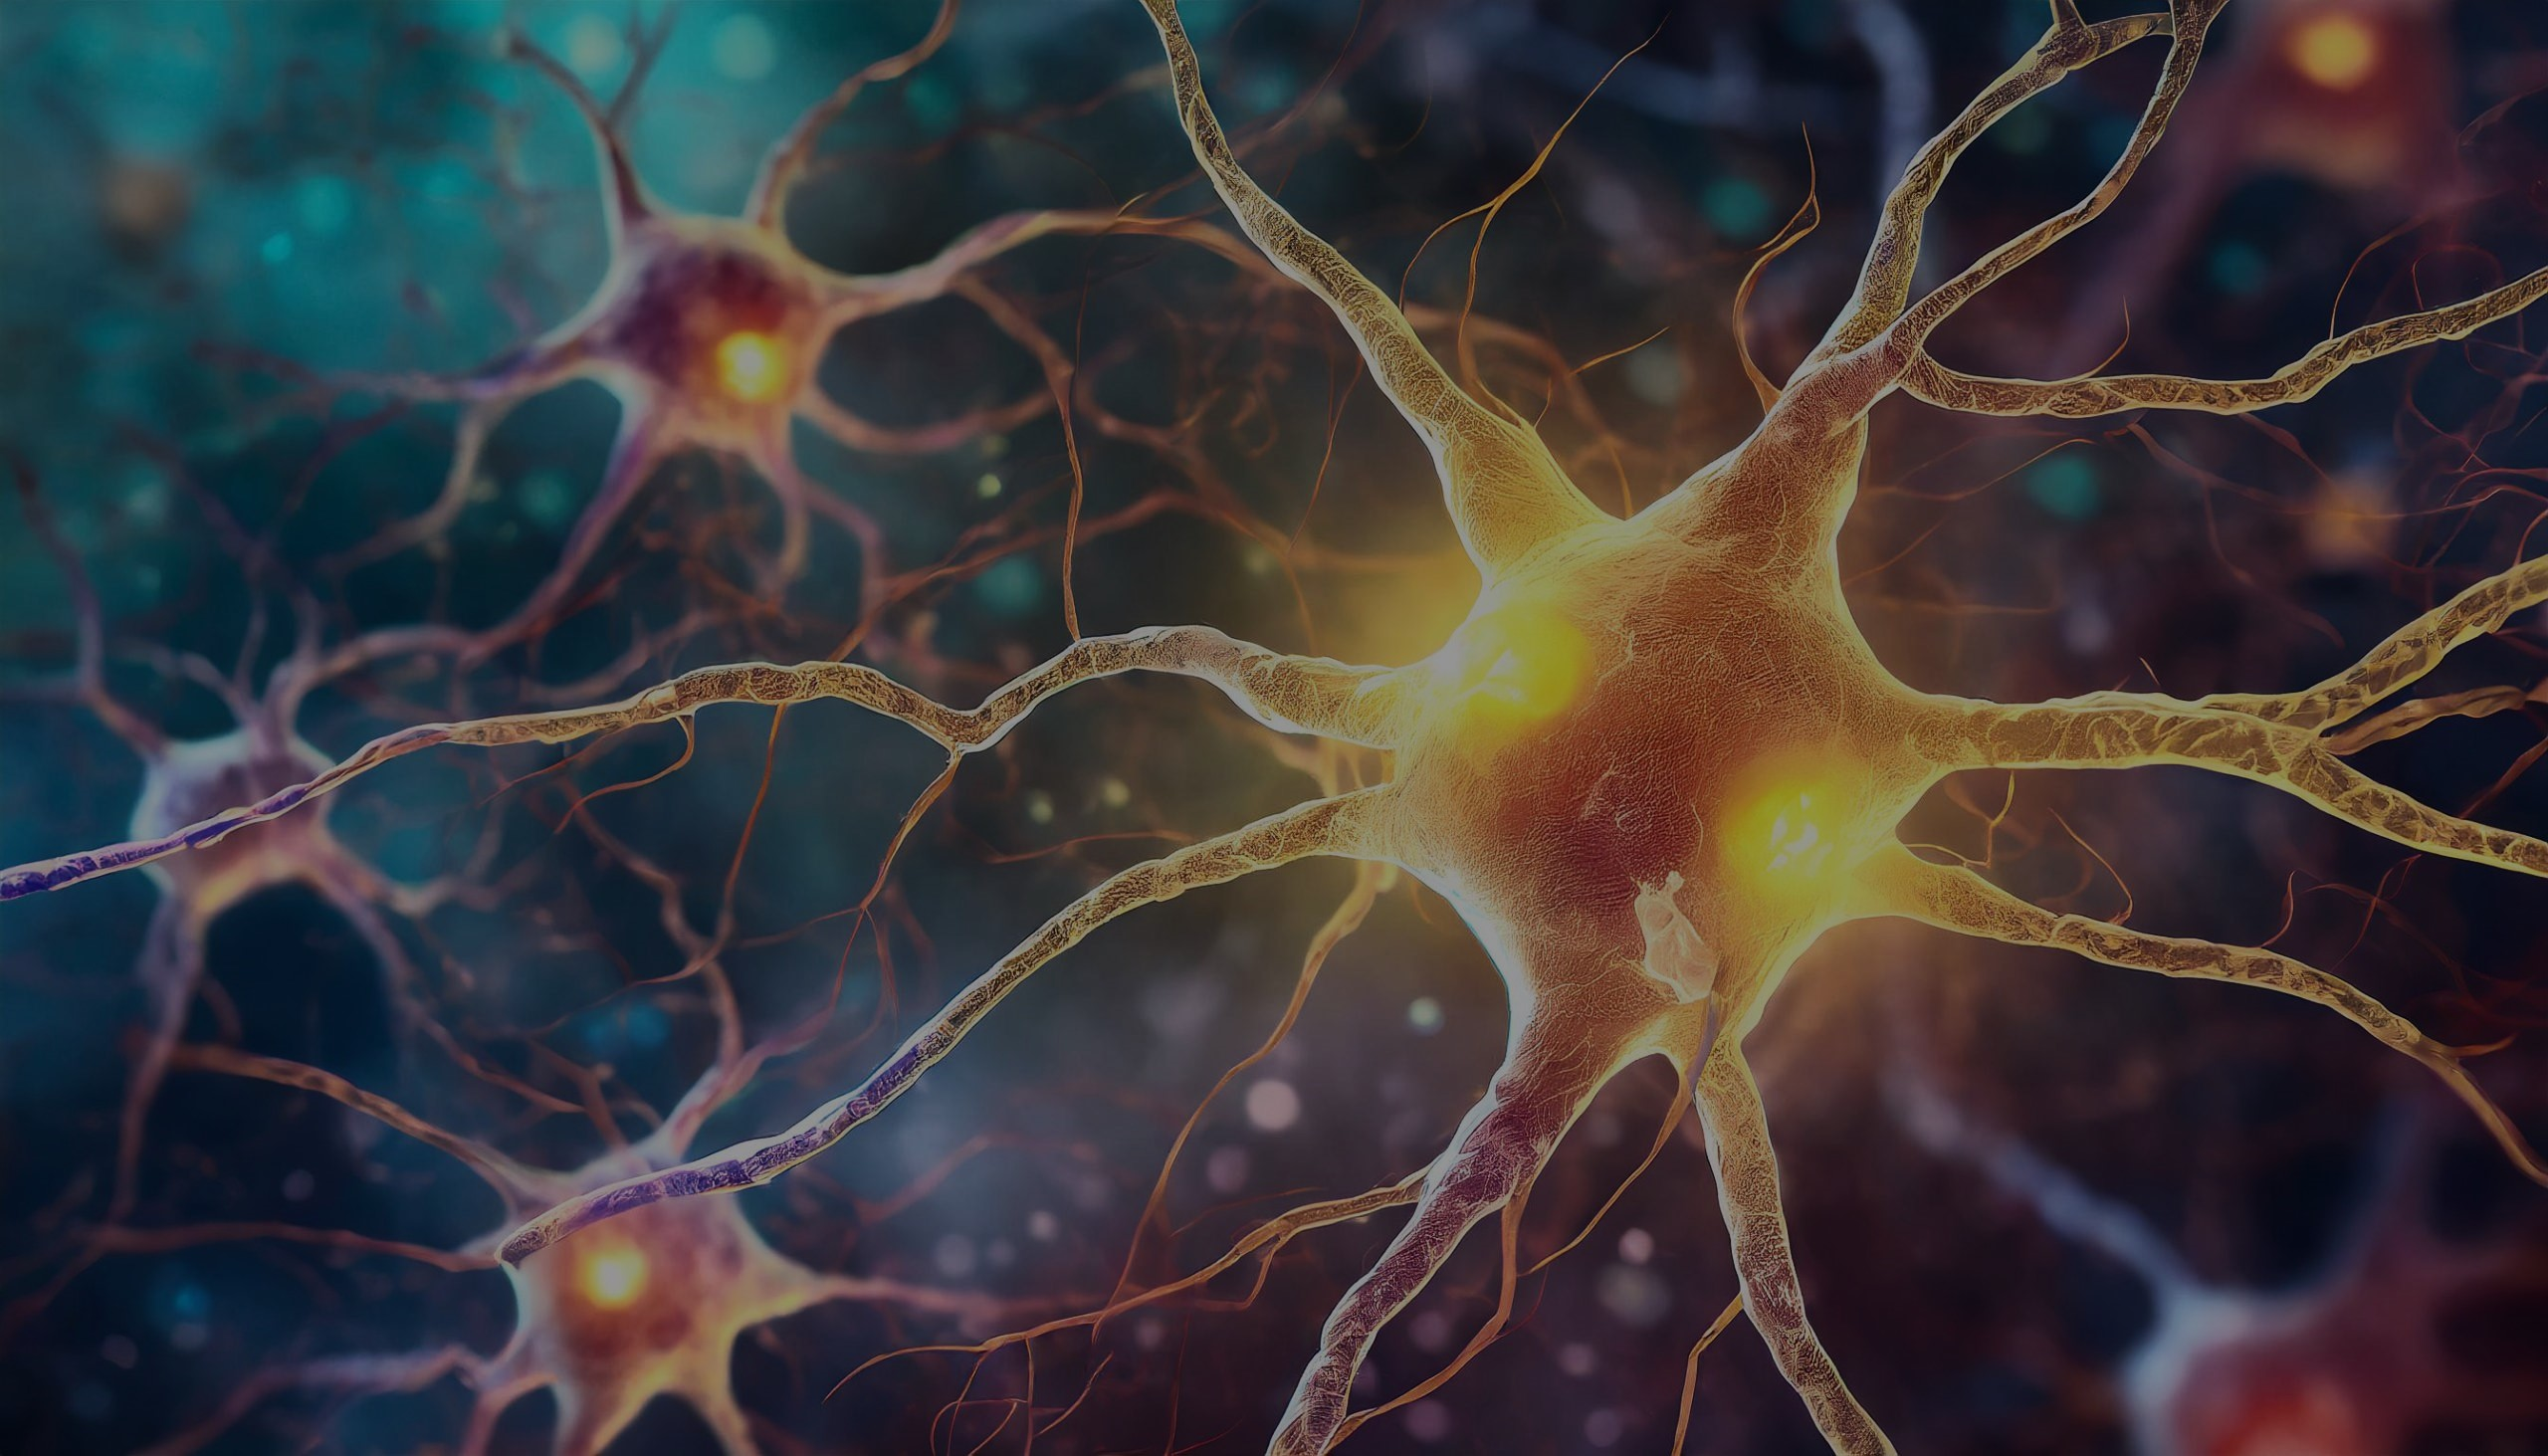
\includegraphics[width=3\paperwidth,height=\paperheight]{abstract_neurons3}
    }%
}


\begin{document}
    \pagenumbering{gobble}
    \begin{titlepage}
        \newgeometry{top=5mm, bottom=10mm, left=15mm, right=15mm}
        \BgThispage
        \color{white} {
            \begin{center}
                \Large \textsc{Matura Thesis}\\Kantonsschule Hohe Promenade\\
                \rule[0.1cm]{16.5cm}{0.1mm}\\
                \vspace{3cm}
                \Huge \textbf{ \textsc{Evolutionary Neural Networks: \\Designing a NEAT-Inspired Algorithm \\for Strategic Game Learning}}\\
                %\vspace{0.8cm}
                %\Large \textit {Implementation and Study of \\Evolutionary Neural Networks}\\
                \vspace{3cm}
                \rule[0.1cm]{16.5cm}{0.1mm}\\
            \end{center}
            \vspace{12cm}\\
            \begin{minipage}[t]{0.47\textwidth}
                \large\textbf {Thesis By:}\\
            \end{minipage}
            \hfill
            \begin{minipage}[t]{0.47\textwidth}
                \raggedleft
                \large\textbf {Lucien Kissling 6e}\\
            \end{minipage}
            \begin{minipage}[t]{0.47\textwidth}
                \large \textbf {Year:}\\
            \end{minipage}
            \hfill
            \begin{minipage}[t]{0.47\textwidth}
                \raggedleft
                \large \textbf {2025}\\
            \end{minipage}
            \begin{minipage}[t]{0.47\textwidth}
                \large \textbf {Supervisor:}\\
            \end{minipage}
            \hfill
            \begin{minipage}[t]{0.47\textwidth}
                \raggedleft
                \large \textbf {Timo Schenk}\\
            \end{minipage}
            \begin{minipage}[t]{0.47\textwidth}
                \large \textbf {Co Examiner:}\\
            \end{minipage}
            \hfill
            \begin{minipage}[t]{0.47\textwidth}
                \raggedleft
                \large \textbf {Dr. Arno Liegmann}\\
            \end{minipage}
            \vfill
        }
        \clearpage
        \restoregeometry
    \end{titlepage}
    Danke an meine Eltern
    Danke an meine Betreuer %TODO: Dankesagung
    Danke an Jan
    \newpage
    \pagenumbering{arabic}
    \setcounter{page}{3}
    \tableofcontents


    \chapter{Introduction}\label{ch:introduction}


    \section{Preface}\label{sec:preface}
    Ever since I got into computer science a few years ago, I was fascinated by the idea of algorithms that solved various problems.
    Therefore, I participated in the SOI (Swiss Olympiad in Informatics) where we were taught everything about developing and programming algorithms and their data structures.
    \\ \\
    In recent years although, a new field of computer science has gained a lot of attention, where these algorithms are not programmed by humans, but evolved by a computer.
    This field called machine learning immediately got my excitement and two years ago a friend of mine and I had our first practical experience with it.
    I developed a simple neural network, which helped us predict the color of a lego brick in front of a color sensor based on the RGB values in various lighting conditions.
    \\ \\
    A neural network (NN) forms the basis of most machine learning models and I will therefore explain it in much detail in the following chapters.
    In simple terms however, a NN is a strongly simplified artificial model of the human brain consisting of an interconnected web of neurons through which information flows and gets computed.
    \\ \\
    Although the NN I developed two years ago already learned on its own, I still had to provide and label data for it to learn from.
    This meant that I had to manually scan the RGB values of the lego bricks and assign them the color they represented.
    In this case, this was the most efficient solution, however there are cases where you train a model where such data is unavailable or you simply want them to develop their own approach for a problem without predefined solutions.
    That is how I got to my matura thesis, which aims to develop such ML models that learn without labeled data with and use those to learn board games.


    \section{Thesis Statement}\label{sec:thesis-statement}
    This thesis explores the field of neural networks (NNs) capable of learning without human-provided data, known as unsupervised learning.
    The focus is on evolutionary neural networks (ENNs), which combine neural networks with evolutionary competition.
    \\ \\
    In this thesis, a simplified implementation of ENNs is developed and trained on board games.
    The research investigates the effects of varying parameters and features on the learning process and evaluates the algorithm’s performance in comparison to other machine learning approaches.
    This project draws inspiration from the NEAT Algorithm, introduced by Kenneth O. Stanley and Risto Miikkulainen in 2002, which uses a minimal initial structure that evolves complexity over time.\footcite[p.105-106]{Neat_02}
    As a benchmark, the ENNs are trained to play the game Nim, where players alternately remove matches from stacks, and the winner is the one who avoids taking the last match.
    \\ \\
    In specific, this Thesis addresses following questions:
    \begin{itemize}
        \item How can evolutionary neural networks (ENNs) be developed that learn to play simple games?
        \item How do different parameters and features of ENNs affect the learning process?
    \end{itemize}


    \chapter{Background}\label{ch:background}


    \section{Neural Networks (NNs)}\label{sec:neural-networks-(nns)}

    As previously mentioned in the Preface, an artificial neural network (ANN or NN) is a mathematical model for data processing, initially inspired by the structure of the brain.
    Therefore, a brief overview of how a brain functions is presented next.

    \subsection{Neurons in the Brain}\label{subsec:neurons-in-the-brain}
    Inside the brain, around 86 million neurons\footcite{caruso_23} form connections to each other through which they activate other neurons with electric and chemical signals.
    In a neuron, the signals of connected neurons add up and when they reach a certain threshold, the neuron is activated and fires a new signal to its own connections\footcite{Newman_23}.
    The neuron then resets after a certain amount of cooldown time.
    \\
    With this web of neurons inside the brain, animals can process the information from nerve signals from the body and output them again as nerve signals instructing the body.

    \subsection{Feed Forward Neural Networks (FNNs)}\label{subsec:feed-forward-neural-networks-(fnns)}
    So how can these ideas about neural networks learned from the biology of a brain applied to a program that runs on a computer?
    The first step is to simplify the chaos of neurons in the brain and organize them into layers of neurons.
    These layers consist of an input layer, an output layer and optional so-called hidden layers in between.
    As a next step, the neurons in each layer are connected to those in subsequent layers, typically limited to connections with the nearest layer.
    \\
    Now, the structure of a neural network looks something like this:
    \begin{figure}[H]
        \centering
        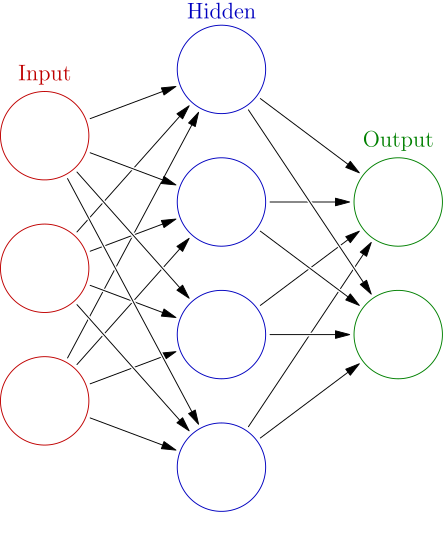
\includegraphics[width=0.25\textwidth]{nn_simple_1}~\caption{A simple Feed Forward Neural Network (FNN) with three layers: Input, Hidden and Output.\footnote{\cite{nn_simple_img_1}}}
        \label{fig:nn_simple_1}
    \end{figure}

    The term topology is used to describe the structure of a NN\@.
    \begin{mydef}{Neural Network Topology}
        The topology of a neural network is its distinct arrangement of neurons, layers and the connections between the neurons.
        \label{definition:Topology}
    \end{mydef}
    For the neural network to perform functions, a weight needs to be assigned.
    This weight value ranges from -1 to 1 and can be thought of as the strength of a connection between neurons.
    \\
    In terms of computer science, this structure now resembles a directed, weighted graph, which is why the neurons are called nodes and their connections edges.
    \begin{mydef}{Nodes/Edges}
        In a neural network, a node receives, computes and sends information, whereas an edge forms the connections between nodes to exchange information.
        \label{definition:Nodes-Edges}
    \end{mydef}
    \\ \\
    The computation process of information by a neural network can be illustrated through the example of a computer vision NN that recognizes digits in a black-and-white image.
    As a first step, the input is encoded into values that correspond to the nodes of the input layer.
    In the example of a computer vision NN, the brightness values of the single pixels might directly represent the nodes of the input layer.
    \\
    Then, the algorithm iterates through all input nodes to identify its connected edges.
    For each of these edges it multiplies its weight by the value of the input node and adds the result to the node on the receiving end.
    \\
    After iterating through all the nodes of one layer, it moves to the next layer.
    At this point, the value of the nodes in the current layer is the sum accumulated by the values of all connected nodes multiplied by the weight of that connection:
    \begin{equation}
        v_x = \sum_{i=0}^{N}v_i * w_i\label{eq:sum_connected_nodes}
    \end{equation}
    Where:
    \textit{
        \begin{itemize}
            \item N is the number of connected nodes
            \item $v_x$ is the value of the current node
            \item $v_i$ is the value of the connected node i
            \item $w_i$ is the weight of the edge connecting the current node to node i
        \end{itemize}
    }

    Additionally, some algorithms add a bias value $r_x$ ranging from -1 to 1 onto the value of the nodes.
    Finally, an activation function $\sigma(x)$ is applied to the value of the nodes to fit the value of the node inside a preferred range.
    This activation function can also be thought of as the threshold of stimulation for a neuron to fire.
    Two examples for activation functions are:
    \begin{itemize}
        \item Sigmoid Function: $\sigma(x) = \frac{1}{1 + e^{-x}}$
        \item Rectified Linear Unit (ReLU): $\sigma(x) = \max{0, x}$
    \end{itemize}
    Plot of the activation functions:
    \\ \\
    \begin{center}
        \begin{tikzpicture}
            \begin{axis}
                [
                xmin=-6,
                xmax=6,
                ymin=0,
                ymax=6,
                ytick distance = 1,
                xtick distance = 1,
                minor tick num=1,
                axis lines = left,
                line width = 1.5pt,
                grid=both,
                major grid style={line width=0.8pt,draw=gray!50},
                minor grid style={line width=0.4pt,draw=gray!20},
                xlabel = \(x\),
                ylabel = {\(\sigma(x)\)}]
                \addplot[
                    domain=-10:10,
                    color=red,
                    samples=1000.,
                ]{1/(1 + e^-x)};
                \addlegendentry{\(Sigmoid\)}
                \addplot[
                    domain=-10:10,
                    color=blue,
                    samples=1000.,
                ]{max(0,x)};
                \addlegendentry{\(ReLU\)}
            \end{axis}
        \end{tikzpicture}
    \end{center}
    \\ \\
    The complete function for the value of one node is therefore:
    \begin{equation}
        v_x = \sigma\left(\sum_{i=0}^{N}v_i * w_i + r_x\right)\label{eq:value_node}
    \end{equation}
    Where (additionally to equation~\ref{eq:sum_connected_nodes}):
    \textit{
        \begin{itemize}
            \item $r_x$ is the bias of the node
            \item $\sigma$ is the activation function
        \end{itemize}
    }

    Now this value $v_x$ is again sent through its connections to nodes in the upcoming layers.
    After iterating through all the nodes and layers of the neural network (NN), the process reaches the final layer of the NN, where the computed output can be read out.
    This output is encoded in node values, as was done with the input, and therefore requires decoding to obtain the final result.
    In the example of a digit-detecting NN, 10 output nodes could be used, each representing one digit.
    The result could then be decoded by identifying the output node with the highest value as the result.
    This kind of output encoding, where all possible results are assigned their own node, is referred to as one-hot encoding.
    With one-hot output encoding, the values of the output nodes can be interpreted as a the neural networks certainty for a specific result to be correct.

    \subsection{Remark: Functioning of NNs}\label{subsec:remark-about-the-funtioning-of-nns}
    Having established how a neural network operates, it is important to understand why this type of algorithm is considered revolutionary in the field of computer science.
    \\ \\
    An algorithm processes an input with a set of functions applied in a certain order to calculate an output.
    Traditionally, a computer algorithm gets programmed with the help of mathematical operations, logic functions, loops, system functions and data structures, which are then converted into binary code for the processor.
    Of course, this also applies in the context of NNs, however, there is also a third layer of abstraction on top, which simulates the functioning of a brain with neurons.
    Since the traditional algorithm only enables the neurons of a NN, the third neuron-based layer is what computes the actual function of the NN\@.
    Therefore, NNs resemble more the functioning of a brain than a traditional algorithm.
    \\ \\
    This difference has implications for the functioning of an NN:
    Traditional algorithms represent actual mathematical calculations and are therefore deterministic.
    With NNs, the algorithm is based on different parameters for nodes and edges, which make it an unpredictable blackbox.
    In the top layer of abstraction, there are no concrete functions but only neuron activation that approximates a function instead.
    This means it is hard to prove a neural network to always be accurate and is also the reason why the result of NNs is often called its prediction.
    \begin{mydef}{NN Prediction}
        The output of a neural network is referred to as its prediction for a given input.
    \end{mydef}

    \subsection{An Example of NN learning: Backpropagation}\label{subsec:an-example-of-nn-learning:-backpropagation}
    It is already established how a neural network with specific parameters generates a prediction for a given input.
    The raises the question: how can parameters encoding the structure, weights, and biases of the neural network be determined?
    The solution lies in using machine learning, which trains the model to perform a specific task using training data.
    \begin{mydef}{Machine Learning}
        Machine learning (ML) is a branch of artificial intelligence that focuses on optimizing artificially intelligent models to solve a given problem.
    \end{mydef}
    One machine learning algorithm for NNs is called backpropagation, which is one of the simplest and most efficient methods to train a NN.\@
    Backpropagation works using a training and test set containing unlabeled data for a problem.
    \begin{mydef}{(Un)labeled Data}
        Labeled data for a machine learning problem is a set of data with sample problems and the respective solutions.
        Unlabeled data instead only contains the sample problems.
    \end{mydef}
    The machine learning process of backpropagation begins with a neural network that has a fixed topology and random weights and biases.
    First, the NN is given the training problems for which it will generate random predictions.
    These random predictions are then refined using the sample solutions.
    This is done by looping back through the NN from the output layer to the input layer, always adjusting the weights and biases in a way that the NN would finally make the right prediction for this problem.
    However, the NN shouldn't be adapted only to a single problem but make accurate predictions for the whole training set and unknown problems.
    To therefore prevent overcorrecting a NN for single problems, a learning rate significantly smaller than 1 is applied to the corrections.
    \\ \\
    The NN is trained on the whole training set for many generations, until the NN starts to make accurate predictions for all problems.
    To evaluate the performance on unknown problems, a separate test set, which the NN hasn't been trained on, can be used.


    \section{Evolutionary Computation (EC) \& Genetic Algorithms (GAs)}\label{sec:evolutionary-computation-(ec)-&-genetic-algorithms-(gas)}
    The focus now shifts to the machine learning technique this thesis focuses on.
    Once again, nature serves as inspiration:
    \begin{mydef}{Evolutionary Computation}
        Evolutionary Computation (EC) is an Algorithm that optimizes a set of parameters for a problem with the help of natural selection.
    \end{mydef}
    Evolutionary computation (EC) is often employed in situations where the optimal parameters for a function cannot be directly calculated, but the performance of a given parameter set can be evaluated.
    One example scenario involves a large dataset of points representing an unknown polynomial function with added noise and outliers.
    To determine the parameters of the underlying polynomial, EC can be utilized to identify the best-fitting parameters.
    The following shows how EC achieves this optimization.
    \\ \\
    The process starts with an initial population of agents with random parameter sets.
    EC then repeats following steps, forming a new generation of the population in each iteration:
    \begin{itemize}
        \item \textbf{Fitness evaluation:} First, EC assesses the performance of each agent, defined by its parameters, in the given problem.
        This performance is referred to as the agent's fitness, which can be evaluated either objectively through a cost function or relatively with a competition between agents.
        In the given example, the cost function might check the prediction of the NN for the given data points, calculate the absolute differences between the prediction and the values of the data points, and use the total sum of these differences as the cost.
        \item \textbf{Selection:} As a next step, the agents that performed well are selected to be part of the next generation.
        \item \textbf{Reproduction:} The selected agents are then replicated by directly copying their parameters (non-mating) or by merging parameters from different agents (crossover).
        \item \textbf{Mutation:} In each new generation, th parameters of the agents are mutated, either by completely replacing certain parameters with new random parameters or by shifting the existing parameters by a random value.
    \end{itemize}
    After a certain number of generations, the EC algorithm will have found best performing set of parameters for a given problem.

    \subsection{Gradient Descent \& Local Minima}\label{subsec:gradient-descent}
    As established in the previous section, EC begins with an initial population of agents with a random set of parameters.
    The fitness of these agents is determined using a cost function.
    Agents with relatively low cost (or high fitness) survive the round and are replicated, mutated and again selected by cost.
    \\ \\
    This whole process strongly resembles a ball rolling down a hill in some terrain.
    At any given point on the terrain, the ball moves in the direction of the steepest descent (ignoring the inertia of the ball).
    Applying this analogy to EC, the parameters for a function can be imagined as the horizontal coordinates for the ball meanwhile the cost of these parameters correspond to the height at that location.
    Mutations produce parameter sets that are close to the original, resembling neighboring points on the terrain.
    As the ball rolls down to the lowest neighboring point in any step, EC again chooses the set of parameters with the lowest cost every cycle.
    This is why the machine learning process is referred to as gradient descent, as the algorithm evaluates all neighboring points and then follows the direction with the lowest cost and therefore steepest gradient.
    \\ \\
    The ball analogy provides insights into the functioning of the EC learning process, which can be understood by visualizing a hill with each a shallow and a deep valley next to it.
    Depending on which side of the hill you place the ball in the beginning, it will roll in a different direction and end up in either of the two valleys, which have different heights.
    Therefore, following things can be derived:
    \begin{itemize}
        \item (Minor) differences in the starting position can result in large differences in the end position and the respective cost.
        \item Once a point with no downwards gradient is reached, innovation halts for that agent, even if there is a point with lower cost somewhere else.
        Such points are called local minima.
    \end{itemize}
    \begin{mydef}{Local Minimum}
        A local minimum is a point with minimal cost compared to its neighboring area and is therefore a halting point for gradient descent.
    \end{mydef}
    The impact of starting position and local minima often pose a large problem for EC applications.
    Strategies to reduce the impact of such are therefore essential for the algorithms success.


    \section{Evolutionary Neural Networks (ENNs)}\label{sec:evolutionary-neural-networks-(enns)}
    After having covered all the basics about neural networks and evolutionary computation, the two concepts are finally combined to create the algorithm this thesis focuses on.
    \begin{mydef}{Evolutionary Neural Networks}
        Evolutionary neural networks (ENNs) are neural networks that use evolutionary computation to optimize for its parameters for the NNs weights/biases and its topology.
    \end{mydef}
    ENNs are useful for complex machine learning problems and also work for unlabeled training data as long as there is a fitness function.
    In the context of neural networks, evolutionary computation can be applied as follows:
    \\
    The parameters encoded by ENNs represent the weights, biases, nodes, and edges of a neural network.
    ENNs still follow the same core process of evolutionary computation:
    They start with a random population of NNs that are evaluated and selected based on a fitness function.
    The selected NNs are replicated (with crossover or non-mating) and finally mutated in following ways:
    \begin{enumerate}
        \item \textbf{Change weights/biases:} A new random value is set for the weight or bias of a random existing edge or node.
        \item \textbf{Shift weights/biases:} The value for an existing weight or bias of a random existing edge or node is altered by a random change but is kept close to the old value.
        \item \textbf{Add edges:} A new edge is added between two random, previously unconnected nodes.
        \item \textbf{Add nodes:} A new node is added in between of a random existing edge.
        The old edge is removed and two new edges with random weights are added between the new node and the two other nodes each.
        \item \textbf{Remove nodes/edges:} A random node or edge is removed in a way that doesn't cut off the input from the output layer.
    \end{{enumerate}}


    \section{Drawing Inspiration from the NEAT-Approach}\label{sec:drawing-inspiration-from-the-neat-approach}
    As already stated in the thesis statement(\ref{sec:thesis-statement}), neuroevolution of augmenting topologies is an ENN machine learning algorithm developed by Kenneth O. Stanley and Risto Miikkulainen in 2002\footcite[p.105-106]{Neat_02}.
    NEAT evolves the topology, weights and biases of NNs at the same time, which makes it particularly suitable for tasks where the optimal network architecture is not yet known.
    One of its key innovations is that the initial population begins with NNs of lowest complexity and the NNs only increase topological complexity as it is useful for the problem.
    In specific, the NEAT algorithm starts with NNs that only have the nodes of the input layer connected to the nodes of the output layer.
    This design aims to produce more efficient neural networks by only increasing complexity when it leads to improved performance.
    The NEAT algorithm therefore only needs the mutations 1. to 4. shown in the last section(\ref{sec:evolutionary-neural-networks-(enns)}) and doesn't need to remove complexity (mutation 5.) as it is already minimal.


    \section{Games}\label{sec:games}
    The following section offers a brief overview of the games on which the ENNs will be trained.

    \subsection{Simple Nim}\label{subsec:simple-nim}
    This game is a simplified version of Nim, where two players take turns removing an arbitrary amount of matches from a single stack with some number of matches.
    The player who removes the last match loses.
    Therefore, the winning strategy simply is to remove all matches from the stack but one, which forces the opponent to remove the last match, which makes them lose.

    \subsection{Nim}\label{subsec:nim}
    This game works similarly to Simple Nim with the difference that there are multiple stacks with matches.
    Now, the player who removes the last match from the last unemptied stack loses.
    The winning strategy for Nim is much more complex, which forces the ENNs to learn a more complex strategy.\footcite{nim_23} %TODO: No wikipedia


    \section{Related Work}\label{sec:related-work}
    The field of AI research in ENNs is largely studied and is often linked to games.
    The following table provides some examples of ENN models that have been tested on games:

    \footnotesize
    \begin{center}
        \hspace*{-2cm}\begin{tabular}{|| l l l l l ||}
                          \hline
                          \makecell{\textbf{Author(s) \& Year}} &
                          \makecell{\textbf{Model}} &
                          \makecell{\textbf{Game/Benchmark}} &
                          \makecell{\textbf{Computation}} &
                          \makecell{\textbf{Accuracy}} \\
                          \hline\hline
                          \makecell{\cite{Neat_02}} &
                          \makecell{NEAT} &
                          \makecell{Double Pole Balancing \\With Velocities} &
                          \makecell{3600 \\evaluations} &
                          \makecell{100\%} \\
                          \hline
                          \makecell{\cite{dama_22}} &
                          \makecell{NEAT} &
                          \makecell{Dama} &
                          \makecell{$>$5000 \\generations} &
                          \makecell{81.25\%\\(wins against humans)} \\
                          \hline
                          \makecell{\cite{go_98}} &
                          \makecell{SANE} &
                          \makecell{Go} &
                          \makecell{260 \\generations} &
                          \makecell{$>$75\%\\(vs Wally, 9$\times$9 board)} \\
                          \hline
                          \makecell{\cite{capture_02}} &
                          \makecell{Custom \\ENN} &
                          \makecell{Capture Game\\(subgame of Go)} &
                          \makecell{$>$100 \\generations\\(distributed)} &
                          \makecell{No significant \\progress yet} \\
                          \hline
                          \makecell{\cite{backgammon_07}} &
                          \makecell{Genetic \\ENN} &
                          \makecell{Backgammon} &
                          \makecell{256 pop,\\100–200 \\generations} &
                          \makecell{62.4\%\\(vs Pubeval)} \\
                          \hline
        \end{tabular}\hspace*{-2cm}
    \end{center}
    \normalsize
    Note:
    Although the amount of fitness evaluations is a more accurate representation of computation load than the amount of generations, in many cases the amount of fitness evaluations isn't indicated and cannot be derived.


    \chapter{Building my ENN}\label{ch:building-my-enn}


    \section{Algorithm Design}\label{sec:algorithm-design}
    This chapter details how to use the concepts described in the last chapter(\ref{ch:introduction}) to build an evolutionary neural network that plays Nim.

    \subsection{Overview}\label{subsec:overview}
    As already mentioned in the thesis statement(\ref{sec:thesis-statement}), this project is written in the Rust programming language\footcite{rust23}.
    The source code and all test data can be found on this thesis' GitHub page\footcite{RustENN}.
    This project utilizes following Rust libraries:
    `rand` (version 0.9.0-alpha.2)\footcite{rand2024},
    `indicatif` (version 0.17.8)\footcite{indicatif2023},
    `csv` (version 1.3.0)\footcite{csv2023},
    `bincode` (version 1.3.3)\footcite{bincode2021},
    `serde` (version 1.0.209)\footcite{serde2024},
    and `rayon` (version 1.10.0)\footcite{rayon2023}.
    The code has been partially written by the AI coding assistant GitHub Copilot\footcite{github_copilot2021}.
    Every instance of artificially generated code has been thoroughly reviewed.
    \\ \\
    The codebase is divided into different modules as well as a bin folder containing main files.
    One module manages the ENN algorithm, while another handles the games that the ENNs are trained to play.
    The ENN module itself is further divided into two files:
    \begin{itemize}
        \item \textbf{agent.rs:} This file handles the NNs and the mutations on the NNs
        \item \textbf{population.rs:} This file handles the natural selection process and data saving
    \end{itemize}
    The game modules provide the problems for the NNs, handle the predictions of the NNs, and find the new game state after a move.
    It further includes an objective performance evaluation function to measure how well the NNs perform.
    \\ \\
    The following sections provide a bottom-up explanation of all functions, beginning with the neural network.
    The implementation uses Rust's structs, which are similar to classes in other programming languages.

    \subsection{Neural Network}\label{subsec:neural-network}
    The struct \textit{NeurualNetwork} (defined in agents.rs) most importantly contains a two-dimensional vector of nodes, which encodes all the information of the NN\@:
    \begin{minted}{rust}
    pub struct NeuralNetwork {
        [...] // redundant side data about the NN
        pub nodes: Vec<Vec<Node>>,
    }
    \end{minted}
    The vector inside (\mintinline{rust}{Vec<Node>}) represents a layer of the NN and the outside vector (\mintinline{rust}{Vec<Vec<Node>>}) contains all layers of the NN\@.
    A \textit{Node} contains its bias and a vector for the incoming and outgoing edges:
    \begin{minted}{rust}
    pub struct Node {
        pub bias: f64,
        //edges stored in an adjacency list
        pub incoming_edges: Vec<Edge>,
        pub outgoing_edges: Vec<Edge>,
    }
    \end{minted}
    An \textit{Edge} contains the weight of the edge and its input/output node:
    \begin{minted}{rust}
    pub struct Edge {
        input: [usize; 2],
        out: [usize; 2],
        weight: f64,
    }
    \end{minted}
    The most important functions of the \textit{NeuralNetwork} struct are:
    \begin{itemize}
        \item \mintinline{rust}{new(input_nodes: usize, output_nodes: usize) -> Self {}}, which initializes the NN with all input and output nodes connected to each other with random weights and biases.
        \item \mintinline{rust}{predict(&self, input: Vec<f64>) -> Vec<f64>}, which computes the output of the NN for a given input with the forward propagation algorithm described in~\ref{subsec:feed-forward-neural-networks-(fnns)}.
        \item \mintinline{rust}{activation_function(x: f64) -> f64}, which computes the neuron activation described in~\ref{subsec:feed-forward-neural-networks-(fnns)}.
        This implementation uses a variant of the \textit{ReLU} function.
        The linearity for inputs greater than zero in the \textit{ReLU} function allows for more variety of neuron activations, enhancing the flexibility and efficiency of the neural network.
        The chosen variant is the \textit{ELU} function, which addresses the issue of dead neurons encountered in \textit{ReLU} by permitting negative output values.
    \end{itemize}

    \subsection{Mutation}\label{subsec:mutation}
    The mutation of the NNs is handled in the \textit{Agent} struct (defined in agent.rs), which includes a NN, its fitness, and its rank:
    \begin{minted}{rust}
    pub struct Agent {
        pub nn: NeuralNetwork,
        pub fitness: f64,
        pub rank: isize,
    }
    \end{minted}
    The function \mintinline{rust}{mutate(&mut self, mutations: usize) -> Self {} } has a number of mutations as a parameter which it applies to the NN of the agent.
    For each mutation, it randomly selects one of the following mutations: Change weights/biases, Shift weights/biases, Add edges, Add nodes.
    All of these mutations have already been described in the last chapter(\ref{sec:evolutionary-neural-networks-(enns)}), although there are some implementation details to mention:
    \begin{itemize}
        \item When inserting a new node in between of two connected nodes (mutation 4.), the inserted node will be added to a random layer in between of the previously connected nodes.
        If the previously connected nodes are in neighboring layers, a new layer is created in between for the new node.
        \item The shift mutation adds to the initial value a random float in the range 0.0 to 1.0 squared with a random sign.
        This gives us following function: \\
        $v_{new} = shift(v_{old}) = v_{old} + rand(-1, 1) * rand_{float}(0..1)^2$
        \item The amount of mutations performed per NN is randomly selected in a range defined by adjustable parameters (see section~\ref{subsec:enn-parameters}).
        \item The type of mutation that is performed is randomly determined for each mutation.
        A weight can be assigned to each mutation as a parameter, which represent its probability to be selected relative to the weights of other mutations (see again section~\ref{subsec:enn-parameters}).
    \end{itemize}

    \subsection{Evolutionary Computation}\label{subsec:natural-slection}
    The EC process starts with an initial population of agents with new, minimal NNs created by the \mintinline{rust}{NeuralNetwork::new()} function (described in \ref{subsec:neural-network}).
    As I already established before (see~\ref{sec:evolutionary-computation-(ec)-&-genetic-algorithms-(gas)}), I now repeat the steps of performance evaluation, selection and mutation.

    \subsubsection{Competition}
    In this case, the fitness evaluation works by letting the agents of a population compete against each other in the games.
    However, I can't let every agent play every other agent since the needed time increases quadratically with population size.
    My solution therefore is to use my circular pairing algorithm.
    This algorithm has a predefined number of opponents each agent needs to play against (see~\ref{subsec:enn-parameters}).
    For each of this predefined number of games, it generates a new distance which it then uses to pair each $\textrm{agent}_i$ with the $\textrm{agent}_{i+distance}$.
    It also checks that the distance isn't a multiple of any distance it had previously since this would result in the same agents being paired twice.
    Each game is played twice with both players starting once while keeping the same initial state.

    \subsubsection{Fitness Evaluation}
    Now, I need to evaluate the fitness of the agents with the fitness function.
    The main idea for the fitness function is to simply count the number of wins an agent has made during the competition.
    Of course, there are other possibilities to evaluate the performance of an agent that represent their performance more accurately.
    The reason why I still first try to use the number of wins as fitness is because it is a generally applicable function to any game.
    Counting the number of wins doesn't require a deeper understanding of the game, which is very useful in games that are indeterministic.
    This also enables the ENNs to find their own new strategy for the game, which is finally the goal of AI training.

    \subsubsection{Natural Selection}
    After the fitness evaluation, I can test the performance of the generation (details in section~\ref{subsec:performance-tests}) and then generate the new population.
    The new population is made up by some portion of each of the following:
    \begin{itemize}
        \item \textbf{Agents from the last generation:}
        The main part of the new population will be drawn from agents from the old generation with high fitness.
        This works by selecting all needed agents randomly using the fitness of my agents as their relative probability of being drawn.
        I can also raise the fitness to some power to either allow more or less survival of non top-performing agents.
        \item \textbf{Random agents from the last generation:}
        Some fraction of the new population is made up of randomly selected agents from the last generation which might help counter a population with the top performing agents stuck in local minimum.
        \item \textbf{New random agents:}
        Another fraction of the new population is made up of newly generated, random agents which might help counter overly complex NNs and also local minima in a population.
        \item \textbf{Old best agents:}
        The last part of the new population is made up of best agents from previous generations which help counter populations stuck in a local minimum.
    \end{itemize}
    Now that I have generated my new population, I can start over the whole process.

    \subsection{ENN Parameters}\label{subsec:enn-parameters}
    As already mentioned in the thesis statement(\ref{sec:thesis-statement}), my research involves testing my implementation with several configurations of different parameters and then evaluate their performance with the stats described in the following section(\ref{subsec:performance-tests}).
    Here is a list of all possible parameters influencing my ENNs:
    \begin{itemize}
        \item \textbf{General:} Size of the population
        \item \textbf{Game:} Initial state of the game, game function that encodes the state for the NN, decodes its prediction, and executes the move on the current state
        \item \textbf{Competition:} Number of opponents per agent
        \item \textbf{Selection:} Fitness exponent, share of old best agents, random agents from last generation and new random agents making up the new population besides agents selected by fitness
        \item \textbf{Mutation:} Min and max amount of mutations per agent, weight/probability of the different mutations
        \item \textbf{Evaluation:} Number of games from the best agent against old best agents

    \end{itemize}
    For each test, I then save a file with the information about the value of all these parameters.

    \subsection{Performance Tests}\label{subsec:performance-tests}
    To see how the Agents perform in the games, I need to track some stats and games.
    I save following data every generation after the competition phase:
    \begin{itemize}
        \item \textbf{Fitness of the best agent:} This stat shows us how much better the best agent performs relatively to the average agent.
        \item \textbf{Wins against older generations:} I pair the best agent against an evenly distributed set of the best agents from past generations to track relative performance to the past.
        As long as this number is above 50\%, I should expect improvement over older generations.
        \item \textbf{Objective grading:} This stat is the performance evaluation of the best agent based on some algorithm that either plays mathematically perfect or (in non-deterministic games) is generally accepted to play well.
        It is important to note that I primarily don't use this algorithm for the fitness function because of the points previously mentioned in section~\ref{subsec:natural-slection}.
        \item \textbf{Number of turns:} I track the average number of turns the agents needed while playing their competition games.
        In Nim, low turn count generally means better play.
        \item \textbf{Average amount of hidden layers and nodes per hidden layer:} I track these stats to see how complex the topologies of my NNs in the population are.
        \item \textbf{Best agent layer sizes and edges:} I track these topological stats to see how complex the best solution is.
        \item \textbf{Best agent games:} I track the whole games turn after turn played by the best agent from the current generation against each the best agent from the last generation and a randomly selected best agent from a previous generation.
        With these game logs, I can see what moves my agents make in real games and try to derive their tactics and strategies.
    \end{itemize}

    \subsection{Nim}\label{subsec:nim-implementation}
    For the nim game, there are a few different game modes as well as an objectively perfectly playing dynamic programming algorithm.
    Let's first look at the general idea of how a game is played.

    \subsubsection{General Approach}
    Each game starts with a first game state, which is derived from the initial state parameter.
    A game state is a list where its length is the amount of stacks in that game and each value $v_i$ stands for the amount of matches on the i-th stack.
    Then, the competing agents take turns predicting their moves.
    On their turn, the active agent reads the current game state as input and predicts its next move.
    A move indicates the stack where the matches are removed as well as the number of removed matches.
    Then the game function computes the new game state after the move or ends the game if all stacks are empty.

    \subsubsection{Encoding and Decoding}
    The input is directly encoded into the input layer of the NNs, which means the input layer has the same size as the state.
    The values of the input nodes are directly copied from the game state list and therefore also represent the amount of matches on each stack.
    \\ \\
    For output encoding, there is two different implementations.
    \begin{itemize}
        \item \textbf{Direct encoding:} I have two output nodes where the value for the first represents the index of the stack and the second value represents the amount of matches that are removed.
        \item \textbf{One-hot encoding:} The first $N$ output nodes encode for the index and the following nodes encode for the amount of matches removed.
        For both the nodes encoding for index and amount removed, the node with the highest value is finally used as output.
        The output layer therefore has length $l = N + \max(state_{initial})$, where $N$ is the amount of stacks and $\max(state_{initial})$ is the highest possible amount of matches on a stack.
    \end{itemize}
    Direct encoding is the more straight forward approach with lower NN topology whereas one-hot encoding ensures that the output stays in a reasonable range.

    \subsubsection{Game Modes}
    There are game modes \texit{Simple Nim} and \texit{Nim} with some configuration possibilities:
    \\
    In \texit{Nim}, each stack of the initial state can hold matches whereas in Simple Nim, the value of all stacks but one randomly chosen stack is set to 0.
    \\
    The stack sizes in the initial state equal the corresponding values from the initial state parameter except for the configuration \textit{random}, where the stack sizes of the initial state are randomly selected with the corresponding values in the initial state parameter as upper bound.
    \\
    Another configuration involves the output decoding.
    With strict grading, illegal moves lead to a game loss, whereas in safe grading, the closest legal move to the illegal prediction is played.

    \subsubsection{Objective Grading}
    To have an exact measure of performance, I use a dynamic programming (DP) algorithm that knows the best moves for each given state.
    It works by first defining a base case, which in case of Nim is every stack being empty and the result a loss.
    Then, it starts with the initial state and tries out all possible moves using recursion.
    For each state it tries to find a move that forces the opponent into a losing position.
    If it can find such a move, the position is winning, but if all moves lead to winning position for the opponent, the algorithm returns the position with the maximal moves needed for the opponent to win.
    It also stores the result for each already computed state, so that all other paths that lead to that position can use the precomputed result.
    \\ \\
    Now that I know for all positions if they're winning, I can use this to grade the moves of my agents:
    For each move, an agent gets one point if
    \begin{itemize}
        \item the agent had a winning state and made a move that got the opponent into a losing state,
    \end{itemize}
    or if
    \begin{itemize}
        \item the agent had a losing state and made a move that required the maximal amount of moves for the opponent to win.
    \end{itemize}
    The sum of all points an agent has collected is then divided by the amount of moves it has made to get the final performance score.


    \section{Findings}\label{sec:first-findings}
    Now I will test my ENN algorithm with the games and different parameters.
    The general approach is to start by training the ENNs on easy problems whilst observing the effect of different parameters on the result.
    Each test is repeated at least 3 times to try to reduce the impact of randomness on the results.
    As I walk through the different testing configurations, I will discuss just one of the tests as long as all tests showed similar results.
    However, all testing data can be inspected on my GitHub.

    \subsection{Simple Nim}\label{subsec:simple-nim-results}
    For the Simple Nim game, I will run each test for 1000 generations, since ENNs should be able to solve this simple game rather quickly.

    \subsubsection{Stack: 2, Configuration 1}
    First I test the ENNs on a problem with one stack containing 2 matches.
    This is the easiest problem one still consider a game - with one match on the stack there is only one legal move, so it doesn't involve much decision-making.
    The winning strategy of course is to only take one match and leave the opponent with the last match on the stack.
    I start my first test with a relatively small population of 100 agents and try to simplify all other parameters:
    \\
    \texttt{game function: run\_nim\_strict}, initial state: \texttt{[2]}, population size: \texttt{100}, competition games: \texttt{50}, mutation min: \texttt{0}, mutation max: \texttt{1}, fitness exponent: \texttt{1}, best agent share:
    \texttt{0}, random agent share: \texttt{0}, random old agent share: \texttt{0}, best agent tournament games: \texttt{50}, add\_connection\_rand: \texttt{1}, add\_node\_rand: \texttt{1}, change\_weight\_rand: \texttt{1}, change\_bias\_rand: \texttt{1}, shift\_weight\_rand: \texttt{1}, shift\_bias\_rand: \texttt{1}\\
    It is also important to note that I start with one-hot output encoding, since this means that the output stays in the desired range.
    \\ \\
    Now, I will run it and see how it goes:
    \\
    \newcommand{\csvpath}{../data/simple_nim/stack_2/t_1/stats.csv} % Rename the macro
    \begin{center}
        \begin{tikzpicture}
            \begin{axis} [
                grid=both,
                xmin=0,
                xmax=50,
                ymin=0,
                ymax=150,
                no markers,
                xtick distance = 10,
                ytick distance = 25,
                legend pos=north west, % Adjust legend position
                xlabel={Generation},
                ylabel={Performance},
            ]
                \caption{Performance of the best agent over generations.}
                \label{fig:sn_stack_1_t_1}
                % First plot
                \addplot table [
                x=generation,
                y=best_agent_avg_performance,
                col sep=comma,
                ] {\csvpath};
                \addlegendentry{\( \text{Best agent perfect play \% (accuracy)} \)}

                % Second plot
                \addplot table [
                x=generation,
                y=best_agent_wins_percentage,
                col sep=comma,
                ] {\csvpath};
                \addlegendentry{\( \text{Best agent wins \%} \)}
            \end{axis}
        \end{tikzpicture}
    \end{center}

    As one can see, the best agent already plays the game perfectly after one generation.
    One can also observe this in my saved games, where the best agent correctly plays the move [0, 1] (first value is the stack, second value the number of matches removed):
    \begin{minted}{}
    Generation: 1
    Best agent layer sizes: [1, 3]
    Agent 1 vs Agent 0:
    Turn: 0: state: [2], agent_move: [0, 1]
    Turn: 1: state: [1], agent_move: [0, 1]
    Game result: [1, 0]
    \end{minted}
    The best agent wins percentage in the plot above is a steady 50\% since all games are played both ways and the first agent always wins the game.

    \subsubsection{Stack: 8, Configuration 1}
    Since the stack size with 2 has already worked fine, I will now try the same configuration with an increased initial stack size of 8 matches:
    \\
    \renewcommand{\csvpath}{../data/simple_nim/stack_8/t_1/stats.csv} % Rename the macro
    \begin{center}
        \begin{tikzpicture}
            \begin{axis} [
                grid=both,
                xmin=0,
                xmax=1000,
                ymin=0,
                ymax=150,
                no markers,
                xtick distance = 200,
                ytick distance = 25,
                legend pos=north west, % Adjust legend position
                xlabel={Generation},
                ylabel={Performance},
            ]
                \caption{Performance of the best agent over generations.}
                \label{fig:sn_stack_8_t_1}
                % First plot
                \addplot table [
                x=generation,
                y=best_agent_avg_performance,
                col sep=comma,
                ] {\csvpath};
                \addlegendentry{\( \text{Best agent perfect play \% (accuracy)} \)}

                % Second plot
                \addplot table [
                x=generation,
                y=best_agent_wins_percentage,
                col sep=comma,
                ] {\csvpath};
                \addlegendentry{\( \text{Best agent wins \%} \)}
            \end{axis}
        \end{tikzpicture}
    \end{center}
    The accuracy of the runs got up to around 30\% and if I look at the games recorded in generation 982, one can see why it didn't get to 100\%.
    \begin{minted}{}
    Agent 998 vs Agent 999:
    Turn: 0: state: [8], agent_move: [0, 2]
    Turn: 1: state: [6], agent_move: [0, 2]
    Turn: 2: state: [4], agent_move: [0, 2]
    Turn: 3: state: [2], agent_move: [0, 1]
    Turn: 4: state: [1], agent_move: [0, 3]
    \end{minted}
    The best agent only learned to play the moves where it subtracts one or two matches.
    This seems quite bad since seemingly all the NNs have to do is to play [0, 7] instantly.
    So why couldn't it learn this one move, when it could do it with stack size 2?
    The problem is that if the starting player subtracts less than 7 matches, the other player would get in winning position where it has to adapt and play subtract N - 1 matches.
    There might evolve a population where all agents only subtract 7 matches, however this seems more like a local minimum and my final goal is to develop NNs that can play the whole game.
    This simplification turns out to be a hindrance, so I will change the stack to have a variable amount of matches.

    \subsubsection{Remark: Unnecessary Topology}
    If I look at the topology metrics of one of the tests, I realize that complexity of the NNs exploded without any visible improvement in performance:
    \begin{center}
        \begin{tikzpicture}
            \begin{axis}[
                title=\textbf{Topology},
                grid=both,
                xmin=0, xmax=1000,
                ymin=0, ymax=50,
                no markers,
                xtick distance = 200,
                ytick distance = 10,
                legend pos=north west,
                xlabel={Generation},
                ylabel={Complexity},
            ]
                \addplot[violet] table [
                x=generation,
                y=avg_layers,
                col sep=comma,
                ] {\csvpath};
                \addlegendentry{Average layers}
                \addplot[teal] table [
                x=generation,
                y=avg_hidden_layer_size,
                col sep=comma,
                ] {\csvpath};
                \addlegendentry{Average hidden layer size}
            \end{axis}
        \end{tikzpicture}
    \end{center}
    I get an average amount of over 20 hidden layers with on average 2 nodes.
    It doesn't make sense for the NNs to have such complexity for such a simple problem as it only increases the needed computations.
    I will therefore reduce the chance for a new nodes and edges to form by a factor of 20 each.
    Let's see if this change impacted the performance and topology of the NNs:
    \\
    \begin{figure}[H]

        \centering
        \pgfplotsset{width=9.5cm,height=6cm,compat=1.18}
        % First graph
        \begin{adjustbox}{valign=c,margin=-2cm 0pt 0pt 0pt} % Shift content left by 2cm
            \begin{minipage}{1.1\textwidth}
                \begin{subfigure}[b]{0.45\textwidth}
                    \centering
                    \begin{tikzpicture}
                        \renewcommand{\csvpath}{../data/simple_nim/stack_8/t_1x/stats.csv} % Rename the macro
                        \begin{axis}[
                            title=\textbf{Performance},
                            grid=both,
                            xmin=0, xmax=1000,
                            ymin=0, ymax=150,
                            no markers,
                            xtick distance = 200,
                            ytick distance = 25,
                            legend pos=north west,
                            xlabel={Generation},
                            ylabel={Performance},
                        ]
                            \addplot table [
                            x=generation,
                            y=best_agent_avg_performance,
                            col sep=comma,
                            ] {\csvpath};
                            \addlegendentry{Best agent perfect play \% (accuracy)}
                            \addplot table [
                            x=generation,
                            y=best_agent_wins_percentage,
                            col sep=comma,
                            ] {\csvpath};
                            \addlegendentry{\( \text{Best agent wins \%} \)}
                        \end{axis}
                    \end{tikzpicture}
                \end{subfigure}
                \hfill
                % Second graph
                \begin{subfigure}[b]{0.45\textwidth}
                    \centering
                    \begin{tikzpicture}
                        \renewcommand{\csvpath}{../data/simple_nim/stack_8/t_1x/stats.csv} % Rename the macro
                        \begin{axis}[
                            title=\textbf{Topology},
                            grid=both,
                            xmin=0, xmax=1000,
                            ymin=0, ymax=50,
                            no markers,
                            xtick distance = 200,
                            ytick distance = 10,
                            legend pos=north west,
                            xlabel={Generation},
                            ylabel={Complexity},
                        ]
                            \addplot[violet] table [
                            x=generation,
                            y=avg_layers,
                            col sep=comma,
                            ] {\csvpath};
                            \addlegendentry{Average layers}
                            \addplot[teal] table [
                            x=generation,
                            y=avg_hidden_layer_size,
                            col sep=comma,
                            ] {\csvpath};
                            \addlegendentry{Average hidden layer size}
                        \end{axis}
                    \end{tikzpicture}
                \end{subfigure}

            \end{minipage}
        \end{adjustbox}
        \caption{Performance metrics over generations in a 2x2 grid.}
        \label{fig:performances-1}
    \end{figure}
    \\
    My modifications didn't impact the performance of the NN, but definitely helped keeping the topological complexity in a reasonable bound.
    I will keep these modifications moving on.

    \subsubsection{Stack 1--8, Configuration 1}
    I will repeat the previous test but with a variable amount of matches between 1 and 8:
    \renewcommand{\csvpath}{../data/simple_nim/stack_8r/t_1.2/stats.csv} % Rename the macro
    \begin{center}
        \begin{tikzpicture}
            \begin{axis} [
                grid=both,
                xmin=0,
                xmax=1000,
                ymin=0,
                ymax=150,
                no markers,
                xtick distance = 200,
                ytick distance = 25,
                legend pos=north west, % Adjust legend position
                xlabel={Generation},
                ylabel={Performance},
            ]
                \caption{Performance of the best agent over generations.}
                \label{fig:sn_stack_8r_t_1.1}
                % First plot
                \addplot table [
                x=generation,
                y=best_agent_avg_performance,
                col sep=comma,
                ] {\csvpath};
                \addlegendentry{\( \text{Best agent perfect play \% (accuracy)} \)}

                % Second plot
                \addplot table [
                x=generation,
                y=best_agent_wins_percentage,
                col sep=comma,
                ] {\csvpath};
                \addlegendentry{\( \text{Best agent wins \%} \)}
            \end{axis}
        \end{tikzpicture}
    \end{center}
    In my tests, the best agent perfect play performance always reaches a value ranging from 40\% to 75\% where it remained stable.
    The NNs were only able to learn the moves where they subtract 1, 2 and 3 matches but no others.
    \begin{minted}{}
    Agent 998 vs Agent 999:
    Turn: 0: state: [6], agent_move: [0, 3]
    Turn: 1: state: [3], agent_move: [0, 2]
    Turn: 2: state: [1], agent_move: [0, 1]
    \end{minted}
    The performance of NNs in different tests just depended on how many moves the NNs learned.
    In any case however, the NNs have got stuck in a local minimum.
    Such local minima originate in an early generations where the agents aren't highly developed, which means they often only play one move.
    The agents that only subtracted one match were therefore the most successful and reproduced the most.
    After reaching that local minimum, there wasn't a competitor that could assert itself, either because of a flaw in the selection process or because none were created in first place.
    One can also see how homogeneous the NNs across generations have become by looking at the wins of the best agent against former best agents, which always settles at 50\%, revealing that they all use the same strategy.
    I will therefore try to modify some parameters to see if anything helps against such local minima.

    \subsubsection{Stack 1--8, Configuration 2--5}
    To overcome local minima, I can use following strategies:
    \begin{itemize}
        \item \textbf{Fitness Exponent:} Increasing the fitness exponent to \textit{ex.} 2 might help successful mutations reproduce better and therefore overcome a large population of similar NNs.
        \item \textbf{Population Composition:} I can add other kinds of agents to the new population like best agents from older generations, randomly selected agents from the last generation, or newly generated random agents.
        This might help the development of new and possibly more complex strategies without the need for instant return in performance.
        \item \textbf{Population Size:} A larger population means more agents with different strategies can exist, evolve and finally help overcoming local minima.
    \end{itemize}
    I now test the effect of these parameters with following 4 configurations:
    \begin{enumerate}
        \item Fitness exponent set to 2
        \item Old best agents, random agents, and new agents each make up 15\% of the population
        \item Population size set to 2500
        \item All parameters combined
    \end{enumerate}
    \begin{figure}[H]

        \centering
        \pgfplotsset{width=9.5cm,height=6cm,compat=1.18}
        % First graph
        \begin{adjustbox}{valign=c,margin=-2cm 0pt 0pt 0pt} % Shift content left by 2cm
            \begin{minipage}{1.1\textwidth}
                \begin{subfigure}[b]{0.45\textwidth}
                    \centering
                    \begin{tikzpicture}
                        \renewcommand{\csvpath}{../data/simple_nim/stack_8r/t_2/stats.csv} % Rename the macro
                        \begin{axis}[
                            title=\textbf{Fitness exponent: 2},
                            grid=both,
                            xmin=0, xmax=1000,
                            ymin=0, ymax=150,
                            no markers,
                            xtick distance = 200,
                            ytick distance = 25,
                            legend pos=north west,
                            xlabel={Generation},
                            ylabel={Performance},
                        ]
                            \addplot table [
                            x=generation,
                            y=best_agent_avg_performance,
                            col sep=comma,
                            ] {\csvpath};
                            \addlegendentry{Best agent perfect play \% (accuracy)}
                            \addplot table [
                            x=generation,
                            y=best_agent_wins_percentage,
                            col sep=comma,
                            ] {\csvpath};
                            \addlegendentry{\( \text{Best agent wins \%} \)}
                        \end{axis}
                    \end{tikzpicture}
                \end{subfigure}
                \hfill
                % Second graph
                \begin{subfigure}[b]{0.45\textwidth}
                    \centering
                    \renewcommand{\csvpath}{../data/simple_nim/stack_8r/t_3/stats.csv} % Rename the macro

                    \begin{tikzpicture}
                        \begin{axis}[
                            title=\textbf{New population composition (each 15\%)},
                            grid=both,
                            xmin=0, xmax=1000,
                            ymin=0, ymax=150,
                            no markers,
                            xtick distance = 200,
                            ytick distance = 25,
                            legend pos=north west,
                            xlabel={Generation},
                            ylabel={Performance},
                        ]
                            \addplot table [
                            x=generation,
                            y=best_agent_avg_performance,
                            col sep=comma,
                            ] {\csvpath};
                            \addlegendentry{Best agent perfect play \% (accuracy)}
                            \addplot table [
                            x=generation,
                            y=best_agent_wins_percentage,
                            col sep=comma,
                            ] {\csvpath};
                            \addlegendentry{\( \text{Best agent wins \%} \)}
                        \end{axis}
                    \end{tikzpicture}
                \end{subfigure}

                \vspace{1em}

                % Third graph
                \begin{subfigure}[b]{0.45\textwidth}
                    \centering
                    \begin{tikzpicture}
                        \renewcommand{\csvpath}{../data/simple_nim/stack_8r/t_4/stats.csv} % Rename the macro

                        \begin{axis}[
                            title=\textbf{Population size: 2500},
                            grid=both,
                            xmin=0, xmax=1000,
                            ymin=0, ymax=150,
                            no markers,
                            xtick distance = 200,
                            ytick distance = 25,
                            legend pos=north west,
                            xlabel={Generation},
                            ylabel={Performance},
                        ]
                            \addplot table [
                            x=generation,
                            y=best_agent_avg_performance,
                            col sep=comma,
                            ] {\csvpath};
                            \addlegendentry{Best agent perfect play \% (accuracy)}
                            \addplot table [
                            x=generation,
                            y=best_agent_wins_percentage,
                            col sep=comma,
                            ] {\csvpath};
                            \addlegendentry{\( \text{Best agent wins \%} \)}
                        \end{axis}
                    \end{tikzpicture}
                \end{subfigure}
                \hfill
                % Fourth graph
                \begin{subfigure}[b]{0.45\textwidth}
                    \centering
                    \begin{tikzpicture}
                        \renewcommand{\csvpath}{../data/simple_nim/stack_8r/t_5/stats.csv} % Rename the macro

                        \begin{axis}[
                            title=\textbf{All combined},
                            grid=both,
                            xmin=0, xmax=1000,
                            ymin=0, ymax=150,
                            no markers,
                            xtick distance = 200,
                            ytick distance = 25,
                            legend pos=north west,
                            xlabel={Generation},
                            ylabel={Performance},
                        ]
                            \addplot table [
                            x=generation,
                            y=best_agent_avg_performance,
                            col sep=comma,
                            ] {\csvpath};
                            \addlegendentry{Best agent perfect play \% (accuracy)}
                            \addplot table [
                            x=generation,
                            y=best_agent_wins_percentage,
                            col sep=comma,
                            ] {\csvpath};
                            \addlegendentry{\( \text{Best agent wins \%} \)}
                        \end{axis}
                    \end{tikzpicture}
                \end{subfigure}


            \end{minipage}
        \end{adjustbox}
        \caption{Performance metrics over generations in a 2x2 grid.}
        \label{fig:performances-2}


    \end{figure}
    As we can see in the graphs, the performance didn't reach 100\% in any configuration and the NNs remained stuck in a local minimum with the best agents always winning 50\% against previous best agents.
    However, there is still something I can change.

    \subsubsection{Stack 1--8, Configuration 6}
    I run the simple configuration as in configuration 1, only that I changed the output encoding (explained in chapter~\ref{subsec:nim-implementation}) from one-hot to direct encoding:
    \\
    \renewcommand{\csvpath}{../data/simple_nim/stack_8r/t_6/stats.csv} % Rename the macro
    \begin{center}
        \begin{tikzpicture}
            \begin{axis} [
                grid=both,
                xmin=0,
                xmax=1000,
                ymin=0,
                ymax=150,
                no markers,
                xtick distance = 200,
                ytick distance = 25,
                legend pos=north west, % Adjust legend position
                xlabel={Generation},
                ylabel={Performance},
            ]
                \caption{Performance of the best agent over generations.}
                \label{fig:sn_stack_8r_t_2}
                % First plot
                \addplot table [
                x=generation,
                y=best_agent_avg_performance,
                col sep=comma,
                ] {\csvpath};
                \addlegendentry{\( \text{Best agent perfect play \% (accuracy)} \)}

                % Second plot
                \addplot table [
                x=generation,
                y=best_agent_wins_percentage,
                col sep=comma,
                ] {\csvpath};
                \addlegendentry{\( \text{Best agent wins \%} \)}
            \end{axis}
        \end{tikzpicture}
    \end{center}
    Now finally got it working!
    The best agent's performance reaches 100\% after 13 generations.
    \\
    So why did the change of output encoding affect the result that heavily?
    \\ \\
    If I look at the NN structure I had a single output neuron for each possible amount of matches I can subtract in one-hot encoding.
    During the evolution process, the connections to the neurons for output 1 and 2 got stronger than the other ones since it lead to a competitive advantage.
    This unfortunately also meant, that the NN was practically unable to adapt to activate the other output neurons.
    In fact, this behavimy would have been entirely predictable, since there is no mathematical way to model an NN that solves this problem with one-hot encoding except for NNs with large amount of hidden nodes.
    Yet NNs with large amount of hidden nodes are unlikely to develop with my ENNs since they don't show a competitive advantage instantly.
    \\\\
    Since this test worked fine, I will now a very large stack size.

    \subsubsection{Stack: 1--1000, Configuration 1}
    Now I will increase the maximal stack number to 1000:
    \renewcommand{\csvpath}{../data/simple_nim/stack_1000r/t_1/stats.csv} % Rename the macro
    \begin{center}
        \begin{tikzpicture}
            \begin{axis} [
                grid=both,
                xmin=0,
                xmax=1000,
                ymin=0,
                ymax=150,
                no markers,
                xtick distance = 200,
                ytick distance = 25,
                legend pos=north west, % Adjust legend position
                xlabel={Generation},
                ylabel={Performance},
            ]
                \caption{Performance of the best agent over generations.}
                \label{fig:sn_stack_1000r_t_1}
                % First plot
                \addplot table [
                x=generation,
                y=best_agent_avg_performance,
                col sep=comma,
                ] {\csvpath};
                \addlegendentry{\( \text{Best agent perfect play \% (accuracy)} \)}

                % Second plot
                \addplot table [
                x=generation,
                y=best_agent_wins_percentage,
                col sep=comma,
                ] {\csvpath};
                \addlegendentry{\( \text{Best agent wins \%} \)}
            \end{axis}
        \end{tikzpicture}
    \end{center}
    The NNs reached full accuracy in less than 30 generations in both the first and second test run.
    However, the NNs got stuck in a local minimum in the third run.
    This is why I also ran other test runs with different parameters but unfortunately, they showed similar consistency within their runs.
    Still, the NNs managed to learn the game most of time which means, I can finally start training the NNs on the main game.

    \subsection{Nim}
    I now already have gained a lot of insight about the functioning of ENNs and are therefore ready for the normal version of Nim.

    \subsubsection{Stacks: 2*2, Configuration 1}
    I will start with a fairly simple problem where there are two stacks containing a maximum of 2 matches.
    There are eight possible game states for which the NNs need to find solutions.
    This shouldn't be a particularly hard task for the NNs so let's see how they do:
    \renewcommand{\csvpath}{../data/nim/stacks_2x2/t_1.2/stats.csv} % Rename the macro
    \begin{center}
        \begin{tikzpicture}
            \begin{axis} [
                grid=both,
                xmin=0,
                xmax=1000,
                ymin=0,
                ymax=150,
                no markers,
                xtick distance = 200,
                ytick distance = 25,
                legend pos=north west, % Adjust legend position
                xlabel={Generation},
                ylabel={Performance},
            ]
                \caption{Performance of the best agent over generations.}
                \label{fig:sn_stack_2x2_t_1}
                % First plot
                \addplot table [
                x=generation,
                y=best_agent_avg_performance,
                col sep=comma,
                ] {\csvpath};
                \addlegendentry{\( \text{Best agent perfect play \% (accuracy)} \)}

                % Second plot
                \addplot table [
                x=generation,
                y=best_agent_wins_percentage,
                col sep=comma,
                ] {\csvpath};
                \addlegendentry{\( \text{Best agent wins \%} \)}
            \end{axis}
        \end{tikzpicture}
    \end{center}
    As expected, the NNs had no problem with this task and in my tests, they reached full accuracy in 100 to 400 generations.

    \subsubsection{Stacks: 2*4, Configuration 1}
    Now I will double the maximal amount of matches per stack which leaves us with 24 possible game states.
    Let's see, how they do:
    \renewcommand{\csvpath}{../data/nim/stacks_2x4/t_1/stats.csv} % Rename the macro
    \begin{center}
        \begin{tikzpicture}
            \begin{axis} [
                grid=both,
                xmin=0,
                xmax=1000,
                ymin=0,
                ymax=150,
                no markers,
                xtick distance = 200,
                ytick distance = 25,
                legend pos=north west, % Adjust legend position
                xlabel={Generation},
                ylabel={Performance},
            ]
                \caption{Performance of the best agent over generations.}
                \label{fig:sn_stack_2x4_t_1}
                % First plot
                \addplot table [
                x=generation,
                y=best_agent_avg_performance,
                col sep=comma,
                ] {\csvpath};
                \addlegendentry{\( \text{Best agent perfect play \% (accuracy)} \)}

                % Second plot
                \addplot table [
                x=generation,
                y=best_agent_wins_percentage,
                col sep=comma,
                ] {\csvpath};
                \addlegendentry{\( \text{Best agent wins \%} \)}
            \end{axis}
        \end{tikzpicture}
    \end{center}
    In all tests did the NNs settle at an accuracy of around 57\% and if I look at the sample games, the NNs demonstrate a clear lack of simple strategy:
    \begin{minted}{}
    Agent 994 vs Agent 995:
    Turn: 0: state: [2, 4], agent_move: [1, 4]
    Turn: 1: state: [2, 0], agent_move: [0, 1]
    Turn: 2: state: [1, 0], agent_move: [0, 1]
    \end{minted}
    The best agent from generation 994 would have had the possibility to force its opponent into a losing position by subtracting two matches from the second stack.
    Instead, it empties the whole stack which leaves the opponent to take all but one matches from that stack.
    \\
    In another game however, the best agent from generation 999 just makes a move that would never be legal in this test:
    \begin{minted}{}
    Agent 999 vs Agent 239:
    Turn: 0: state: [4, 3], agent_move: [1, 5]
    \end{minted}
    It is hard to tell if this is a result of the NNs being in a local minimum or because of to little training so I will run the tests a bit longer to give the NNs more chances to develop.
    %Another thing that stands out is that the NNs tended to develop a lot of unnecessary topological complexity which is why I will decrease the chance for node growth again by a factor of 5.
    %\section{Direct Comparisons}

    \subsubsection{Stacks: 2*4, Configuration 2}
    I will run the tests for 10'000 generations instead of 1000:


    \chapter{Wrapping Up}\label{ch:wrapping-up}


    \section{Conclusion}\label{sec:conclusion}
    I managed to train neural networks with 100\% accuracy in the simple Nim version, where there is only one stack, for stack sizes up to 1000.
    This success was mostly due to the realization that the output should be encoded directly instead of using one-hot encoding.
    Although one-hot encoding keeps the output in a safe bound, it finally makes it harder for the NNs to find the correct structure and weights in the case of Nim.
    Other parameter configurations were explored, however, most of them showed to be similarly effective as the initial configuration, except for the weight reduction of topology increasing mutations which showed to be effective.
    In the full Nim game, the NNs were able to reach an accuracy of 100\% for two stacks with two matches each but only reached an accuracy of ~60\% for two stacks with 4 matches each.
    Since the NNs already weren't able to understand this problem, it didn't make sense to train them on even more complex configurations.
    \\\\
    There are two possible explanations for the failure to develop accurate NNs in the Nim game.
    Either, the Nim game is a bad game for NNs to solve since the algorithm to play Nim perfectly isn't easily translatable into neurons, or my implementation and or parameters of the ENN simply wasn't up to the task.
    To tell which of the two reasons apply, there needs to be done more research in this field, which will be discussed in the last section (\ref{sec:future-work}).
    \\ \\
    This thesis also showed sometimes contradictory results within different tests of the same parameters.
    In an application, one might therefore train several populations to then choose the best performing one.


    \section{Auto Review}\label{sec:auto-review}
    This research was a large and sometimes painful journey for me to realize but finally resulted in a ENN framework that I proved to be able to learn some functions without human help.
    Still, there is a few things I would do differently.
    \\
    I planned to be done with a beta program many months before the thesis end to then have time to test and refine my program.
    However, I finished the program much later and found many bugs which forced me to repeat the whole testing.
    The final tests were therefore done in only a few days, which left me with little room to search for optimal parameters.
    Additionally, my implementation wasn't optimized for speed, which further increased the time problem.
    \\
    Another thing I realized is that a scientific approach helps a lot with finding a solution.
    I first had fixed ideas about certain features and parameters and only realized these ideas were flawed after starting with a simple solution and then testing different approaches one at a time.
    \\
    I would also do some things differently in terms of my implementation.
    Firstly, I had many confusions with parameters which I had defined all over the place in my project.
    I would create a struct that handles all parameters and implement automized testing so I could run all tests without my supervision.
    \\
    However in general, my object oriented programming approach worked fine and my project structure made it easily understandable and editable throughout my research.
    Still, more consistent commenting and documentation would have further improved clarity of the code.


    \section{Future Work}\label{sec:future-work}
    As already mentioned, this thesis leaves much research to be conducted, which might also answer the question whether the Nim game can be played by NNs.
    In specific, future work might include the following:

    \subsubsection{More Testing}
    Because of the time constraints, this research only tested few configurations with little tests each.
    More test runs within a set of parameters might therefore increase statistical significance of the results and more tests with different sets of parameters might help find better solutions.
    One might also use evolutionary computation to optimize different parameters of the ENNs.

    \subsubsection{Faster Computation}
    To enable more tests, one could improve the computation performance of the ENN algorithm.
    This can be done by converting the NNs into a weight matrix and then compute its predictions with hardware accelerated vector matrix multiplications.
    However, the complex topologies of the NNs in this approach make it harder to do so than with other NNs.
    Also many small performance improvements can still be done in this project which might cumulatively make it drastically faster.

    \subsubsection{Algorithm Design}
    There are also a lot of improvements to be made in the ENN algorithm, this thesis developed.
    For example, the NEAT algorithm, which served as initial inspiration, also uses genetic encoding, tracks genes using historical markings and protects innovation using speciation\footcite{Neat_02}.
    All of these and other approaches could improve the ENNs performance and therefore need to be studied.
    %\subsubsection{Tests in different Applications}
    %To test the ENNs performance, one might also use this implementation for other applications to see if it holds up against different ENN algorithms.
    %\chapter{Appendix}
    %    \section{Data}
    %Possibly additional tests
    %    \section{References}
    \printbibliography[title=References]

\end{document}
